%!TEX root = ../thesis.tex

\thispagestyle{myheadings}

\graphicspath{{Body/Figures/ExperimentalOverview/Auxiliary/}{Body/Figures/ExperimentalOverview/Calorimeter/}{Body/Figures/ExperimentalOverview/Ring/}{Body/Figures/TrackingFigures/TrackerPics/}{Body/Figures/ExperimentalOverview/Ring/}{Body/Figures/TrackingFigures/CoordSys/}{Body/Figures/TrackingFigures/Drift/}{Body/Figures/TrackingFigures/Electronics/}}

\chapter{Detector Systems}
\label{sec:DetectorSystems}

While the calorimeters are the primary detector and gather the most data to measure the \wa signal, there are a number of different auxiliary systems for monitoring injection and beam dynamics. These include the T0, IBMS, and fiber harps. The straw tracking detectors measure beam dynamics, but also serve as a cross check for some parameters of the calorimeter, and are used to look for a possible EDM signal. (Haven't mentioned EDMs at all at this point so maybe leave this last bit out.) Each of these systems will be described in the following sections.


\section{Auxiliary detectors}

\subsection{T0}
\label{sec:T0}

During data taking, a reference time must be chosen so as to align all different detector systems in time. When taking data from fill to fill, decay positron spectra must be aligned in phase. Without this functionality, analyzing the data from different systems and comparing them would be impossible. To do this a ``T0'' counter is placed just on the outside of the ring before the inflector. It is made up of a scintillating paddle connected to two photo-multiplier tubes (PMTs) \cite{t0Hannah,t0Aaron}. See \figref{fig:T0counter}. One PMT, PMT A, has a 1\% neutral density filter resulting in low photo-electron stats, and acts primarily as a timing measurement. The other, PMT B, has a 10\% neutral density filter resulting in higher stats, and acts as a shape counter and proxy for fill intensity. (In general the signals are very similar.) Together they provide a measure of the injected beam profile in time, allowing to align the detectors each fill, and the data from fill to fill. Some measured T0 pulses are shown in \figref{fig:T0pulses}. The shape of the incoming pulses has a somewhat trident-like shape, with a very large spike in the middle of the time width, and two spikes on the outside edges. This shape owes itself to the accelerator complex, and varies from bunch to bunch.


\begin{figure}[]
\centering
    \begin{subfigure}[t]{0.45\textwidth}
        \centering
        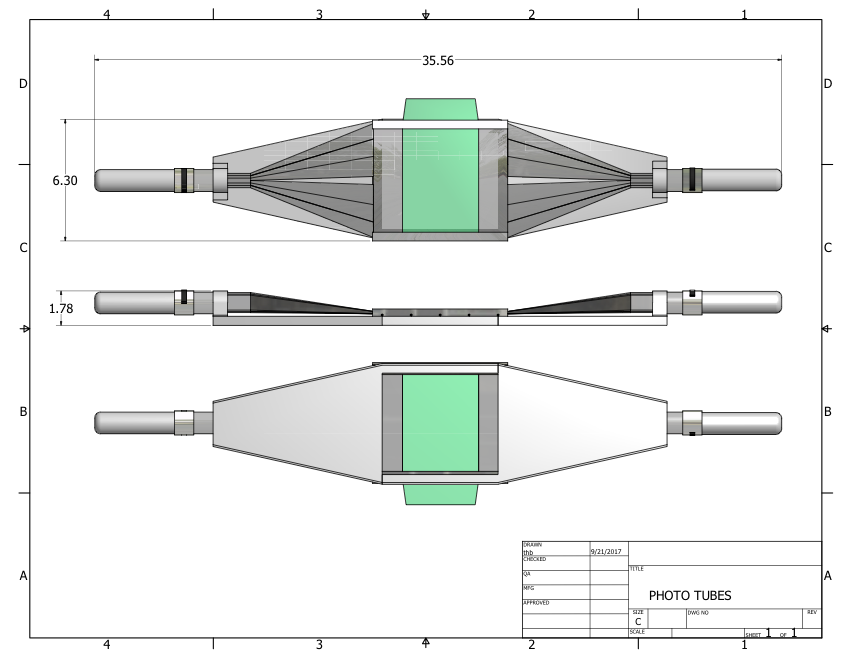
\includegraphics[width=\textwidth]{T0}
        \caption{The T0 counter is made up of a scintillator in the middle shown in green, which connects with light guides to PMTs on the left and right.}
    \label{fig:T0counter}
    \end{subfigure}%
    \hspace{1cm}
    \begin{subfigure}[t]{0.45\textwidth}
        \centering
        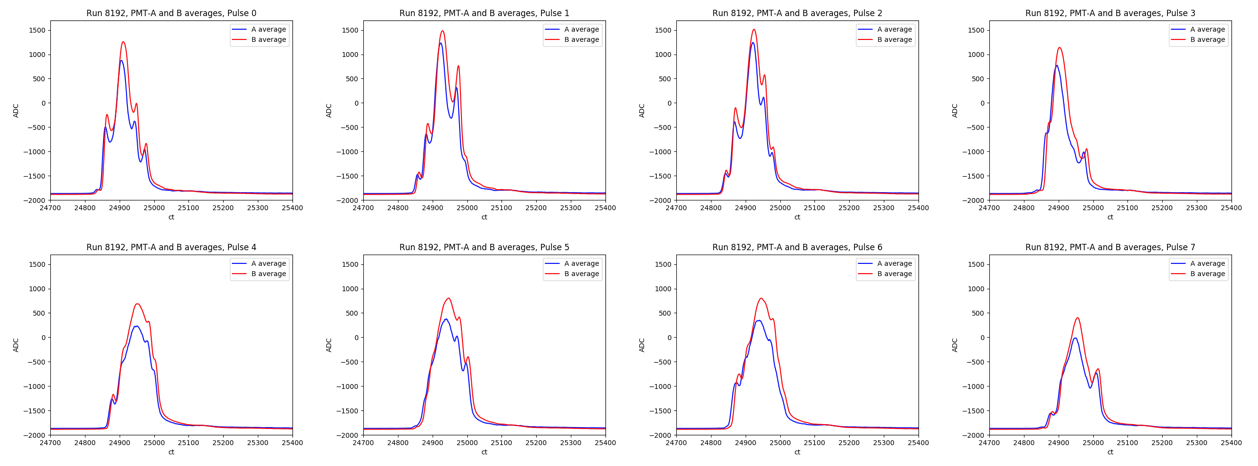
\includegraphics[width=\textwidth]{T0pulses}
        \caption{Time profiles for the two PMTs in the T0 counter for one of the eight bunches we receive at a time as described in \secref{sec:Accelerator}. Each profile is an average of 100 such profiles. The x axis is in clock ticks, each of which is $\SI{1.25}{ns}$.}
    \label{fig:T0pulses}    
    \end{subfigure}
\caption[T0 counter and pulses]{Figures from \refref{t0Hannah}.}
\label{fig:T0}
\end{figure}


\subsection{Inflector Beam Monitoring System}
\label{sec:IBMS}

While the T0 provides timing and intensity measurements, the inflector beam monitoring system (IBMS) provides measurements of the beam position properties as it passes through the inflector. This is useful because the injection aperture is so tight, and incoming beam parameters are tightly constrained. The IBMS system serves to provide a direct diagnostic handle on the phase space matching between the last accelerator components and the \gmtwo storage ring \cite{ibms1}. The IBMS is made up of two scintillating fiber detectors, as shown in \figref{fig:IBMS1and2}. These devices are placed at the outside of the magnet yoke before injection into the back hole of the magnet, and at the entrance to the inflector \cite{ibms2}. A third device is planned to be at or near the downstream end of the inflector. See \figref{fig:IBMSPlacement}. 


\begin{figure}[]
    \centering
    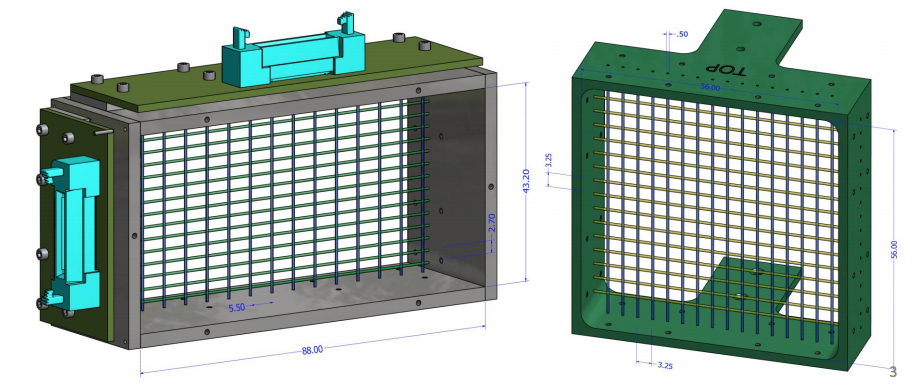
\includegraphics[width=0.9\textwidth]{IBMS1and2}
    \caption[IBMS Models]{Simulation models of the IBMS 1 and 2 detectors. Scintillating fibers form an array which detect particles as they pass through them.}   
    \label{fig:IBMS1and2}
\end{figure}

\begin{figure}[]
    \centering
    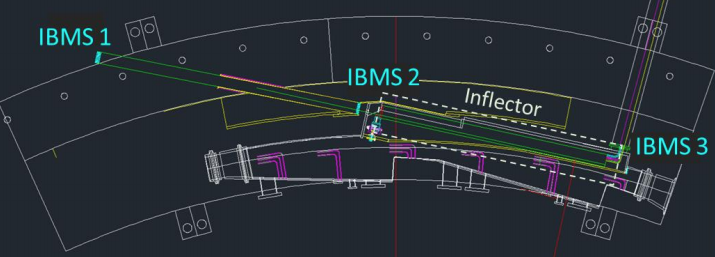
\includegraphics[width=0.9\textwidth]{IBMSPlacement}
    \caption[IBMS Positions]{The positions of IBMS 1, 2, and the planned 3rd device are shown with respect to the vacuum chamber and inflector.}   
    \label{fig:IBMSPlacement}
\end{figure}



\subsection{Fiber Harps}
\label{sec:FiberHarps}

The last auxiliary detector is the so called ``fiber harp'' system. It is made up of four scintillating fiber detectors located within the ring that serve to measure the beam intensity as a function of time and position \cite{fiberharp}. Two of the detectors measure the radial components of the beam, and two measure the horizontal components. The fiber harps are located at points 180\textdegree{} and 270\textdegree{} from the inflector. One of these devices is shown in \figref{fig:fiberharp}. The fiber harps have the added advantage that they are able to measure beam properties throughout the fill, providing a diagnostic tool which is sensitive to the scraping procedure and the CBO properties of the beam. An example of fiber harp measurements is shown in \figref{fig:fiberharp_measurement}. However because the fiber harps are a destructive measurement of the beam due to multiple scattering in the fibers, the system was designed to be retractable. They are inserted during special diagnostic or systematic runs, and are pulled out of the beam path during production data taking.


\begin{figure}[]
\centering
    \begin{subfigure}[t]{0.45\textwidth}
        \centering
        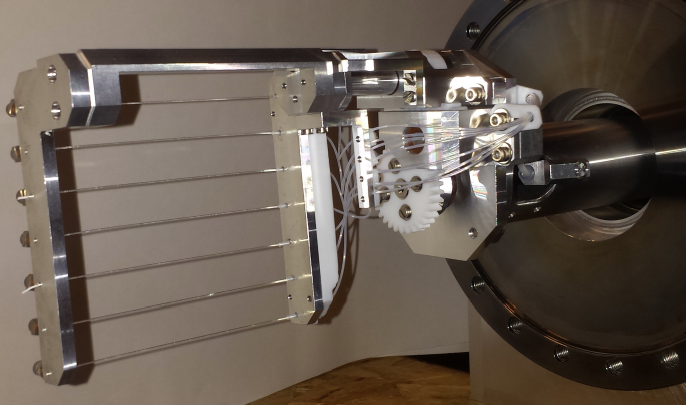
\includegraphics[width=\textwidth]{fiberharp}
        \caption{Picture of one of the fiber harps. A row of seven scintillating fibers measures the beam intensity as a function of time at vertical or horizontal positions depending on which fiber harp is inserted.}
    \label{fig:fiberharp}
    \end{subfigure}%
    \hspace{1cm}
    \begin{subfigure}[t]{0.45\textwidth}
        \centering
        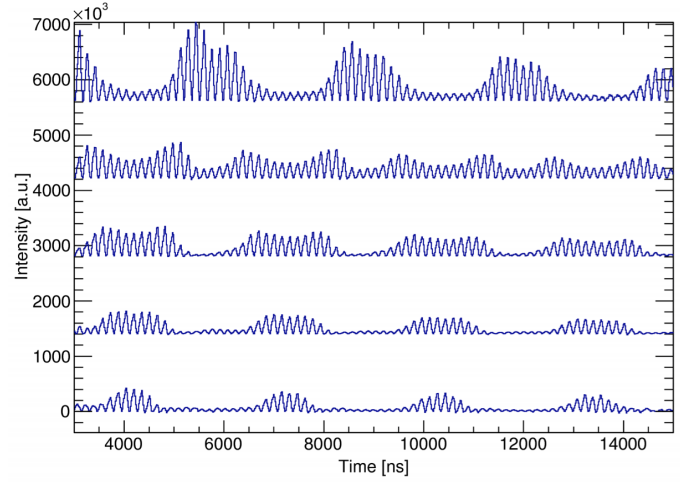
\includegraphics[width=\textwidth]{fiberharp_measurement}
        \caption{Shown are fiber harp beam intensity measurements for the horizontal fiber harp. Each spectra is from a single fiber, with the spectra at the top being at the greatest radial positions. The fast oscillations of the cyclotron frequency can be seen along with the slower oscillations of the CBO.}
    \label{fig:fiberharp_measurement}
    \end{subfigure}
\caption[Fiber harp and measurement]{Fiber harp related pictures.}
\label{fig:fiberharppics}
\end{figure}





\section{Calorimeters}
\label{sec:Calorimeters}


Electromagnetic calorimeters are the primary detector in the E989 experiment, responsible for the \wa measurement. They measure hit times and energies of decay positrons as they curl inward from the storage region. 

\subsection{Requirements and systematic effects}

In order to determine \wa to the precision goal, there are specific requirements on the performance of the calorimeters. First, they must have a relative energy resolution of better than 5\% at $\SI{2}{\GeV}$, in order for proper event selection above threshold \cite{TDR}. The energy resolution requirement is modest but not strict because the important observable is the number of detected positrons above some energy threshold, where the energy threshold can be determined emperically.

Second, they must have a timing resolution of better than $\SI{100}{ps}$ for positrons with greater than $\SI{100}{\MeV}$ \cite{TDR}. The calorimeters must be able to resolve multiple incoming hits through temporal or spatial separation at 100\% efficiency for time separations of greater than $\SI{5}{ns}$, or 66\% of hits for time separations less than $\SI{5}{ns}$, in order to reduce the pileup systematic effect. Pileup is the term used for when multiple particles impact the detector within the deadtime of the detector such that they are registered as a single hit. Unresolved pileup means that the number of detected positrons above threshold is mis-measured. Since pileup is a time-dependent effect, where pileup decays at some lifetime approximately equal to half the muon lifetime, this leads to a mis-measurement of \wa. The requirements stated here assist in reducing the pileup systematic error below the target goal of $\SI{40}{ppb}$.

Third, the energy response of calorimeters for measured hits must be stable to $< 0.1\%$ over a fill (\mus{700}) \cite{TDR}. The long term energy response stability over a time period of order seconds must be $< 1\%$. The energy response of a detector as a function of time is typically referred to as the gain of the detector, where technically the gain refers to the amount of current output per detected hit. The gain depends on the temperature stability and hit rate. After a hit, the measured energy fraction of a following hit drops sharply and then rises exponentially back to one. This is referred to as the short-term double pulse (STDP) effect. At injection many particles are injected into the ring and there is a large amount of secondary particles incident in the calorimeters. The accumulation of all the individual STDP effects ends up causing a large gain drop at the beginning of each fill. This is typically referred to as the in-fill gain (IFG) effect. Hits with mis-measured energies due to these effects can thus be excluded from the fitted histogram if their energies drop below threshold, leading to another systematic effect and subsequent error in the \wa measurement. (Temperature changes vary over time scales greater than a fill, so don't contribute to the systematic error.) The requirements stated here, along with the use of a laser calibration system (\secref{sub:LaserCalibrationSystem}), assist in reducing the gain systematic error below the target goal of $\SI{20}{ppb}$.



\subsection{Harware}


There are 24 calorimeters located symmetrically around the inside of the ring placed flush to the vacuum chamber wall, as shown in \figref{fig:CalorimeterPositions}. (Indeed the shape of the vacuum chambers were designed so as to reduce multiple scattering of the decay positrons before entering the calorimeters.) Each calorimeter sits on a board extending out from a cart which contains the electronics that power the calorimeters and read out the data. The carts help to relocate magnetic materials away from the field region to avoid perturbing the magnetic field, and provide easy access to the electronics while removing them from the positron decay path region.


Each calorimeter consists of 54 channels of PbF\textsubscript{2} crystals arrayed in a 6 high by 9 wide array, for a total of 1296 channels. Each crystal is $2.5 \times 2.5 \times 14$~cm\textsuperscript{3} and is wrapped in black Tedlar\textregistered\ foil. The PbF\textsubscript{2} material has an index of refraction of 1.8, and emits Cerenkov light as incident positrons with energy greater than $\SI{100}{\keV}$ pass through the crystals \cite{Fienberg:2014kka}. Cerenkov light is naturally fast which improves the timing resolution of the incoming hits. The high density of the PbF\textsubscript{2} gives it a short radiation length, such that the energy deposition from the incident positrons is nearly 100\% over the length of the crystal. The black foil is used to reduce light transmission between crystals and improve position reconstruction, as well as reduce pulse width \cite{Kaspar:2016ofv}. The energy deposition from the incident positrons is typically restricted to only one or two crystals. The segmentation of the calorimeter combined with the black wrapping helps the spatial and temporal resolution of the detected pulses. See \figref{fig:CalorimeterCrystals} for a picture of the calorimeter crystals.


\begin{figure}[]
\centering
    \begin{subfigure}[t]{0.45\textwidth}
        \centering
        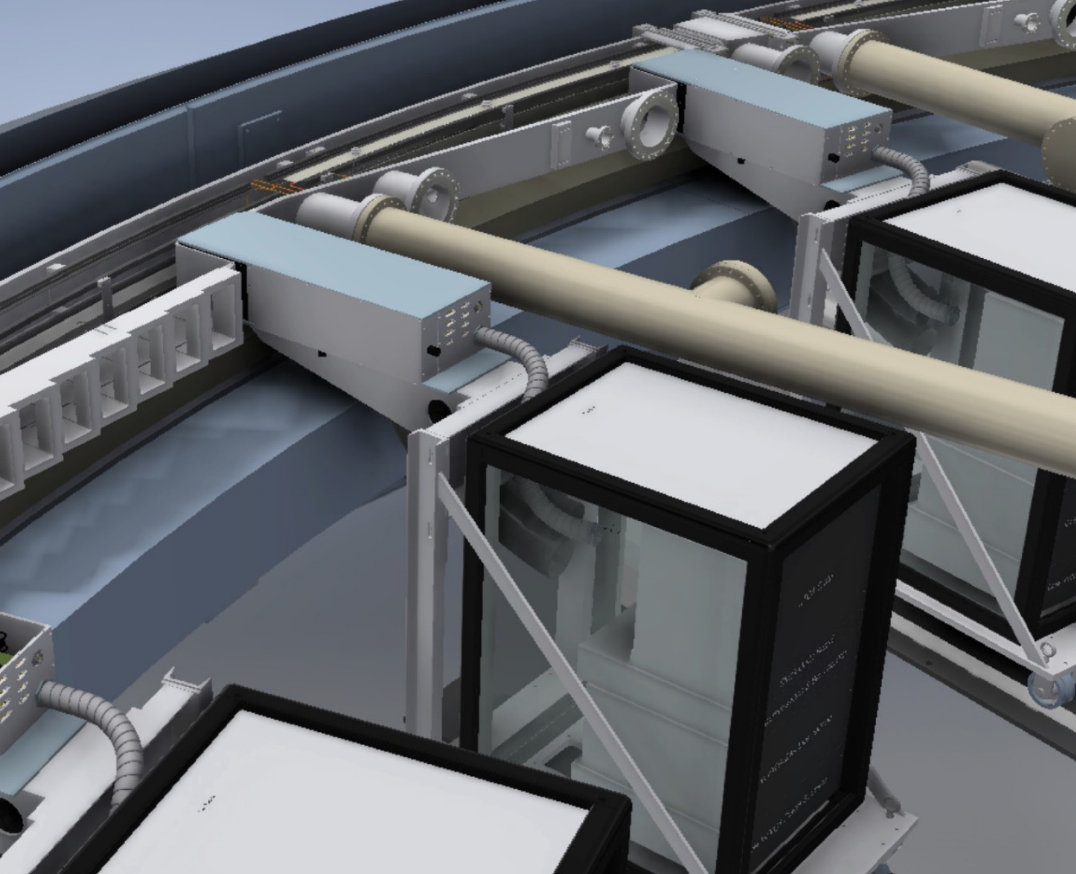
\includegraphics[width=\textwidth]{CalorimeterPositions}
        \caption{In black are the calorimeter carts, which house the electronics for the calorimeters. They hold up a board upon which the calorimeter rests. The calorimeter as shown is pushed flush to the vacuum chamber on the left.}
    \label{fig:CalorimeterPositions}
    \end{subfigure}%
    \hspace{1cm}
    \begin{subfigure}[t]{0.45\textwidth}
        \centering
        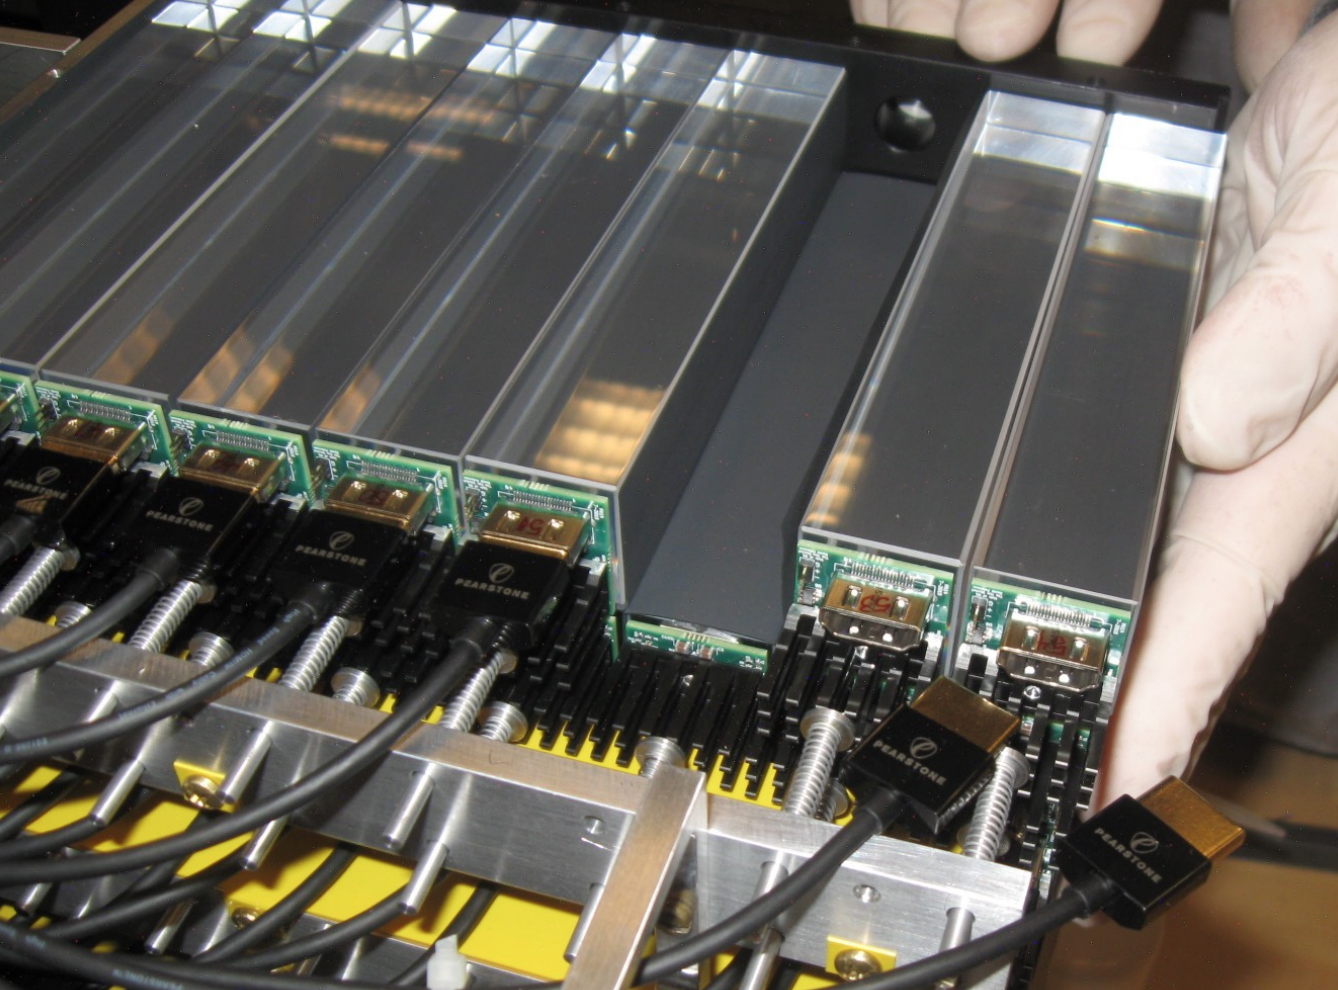
\includegraphics[width=\textwidth]{CalorimeterCrystals}
        \caption{Shown is the backside of a calorimeter. The clear blocks are the PbF\textsubscript{2} crystals, each of which has a SiPM mounted onto the back of them.}
    \label{fig:CalorimeterCrystals}
    \end{subfigure}
\caption[Calorimeters]{Calorimeter systems relative to the vacuum chamber (left) and an individual calorimeter (right). \bf{probably update these pictures at some point}}
\label{fig:calos}
\end{figure}



Each crystal is paired with a large area silicon photo-multiplier (SiPM) sensor which reads out the emitted Cerenkov light. SiPMs are compact, operable in high magnetic field regions, have very linear responses for operation at MHz rates, are suited to measuring Cerenkov light due to their high photo-detection efficiency in the wavelengths of interest, and have a high degree of gain stability \cite{Kaspar:2016ofv}. The SiPMs used are designed by Hamamatsu and detailed in \refref{Kaspar:2016ofv}. They sit on printed circuitry boards (PCBs) devoid of magnetic materials, which are designed to preserve the fast SiPM pulse shape. The combined properties of the chosen SiPMs, their electronic boards, and the PbF\textsubscript{2} crystals results in an energy resolution of $(4.6 \pm 0.3) \% / \sqrt{E/\GeV}$, a timing resolution of $\SI{20}{ps}$, and a pulse width of $\SI{5}{ns}$, satisfying the stated requirements earlier \cite{Fienberg:2014kka,Kaspar:2016ofv}. Details of the pulse fitting algorithms are shared in \secref{sec:ReconWest}. The SiPMs can be seen in \figref{fig:CalorimeterCrystals}. Finally, 12-bit waveform digitizers (WFD) sample each SiPM channel at a rate of 800 mega-samples per second with a 1 Gb memory buffer and the data are transferred to a bank of GPU processors for on-line data processing \cite{Sweigart:2016jty}. The timing resolution of these WFDs is $<\SI{50}{ps}$ for most pulse amplitudes. A typical pulse from an incident positron is shown in \figref{fig:calopulse}.

\begin{figure}[]
\centering
        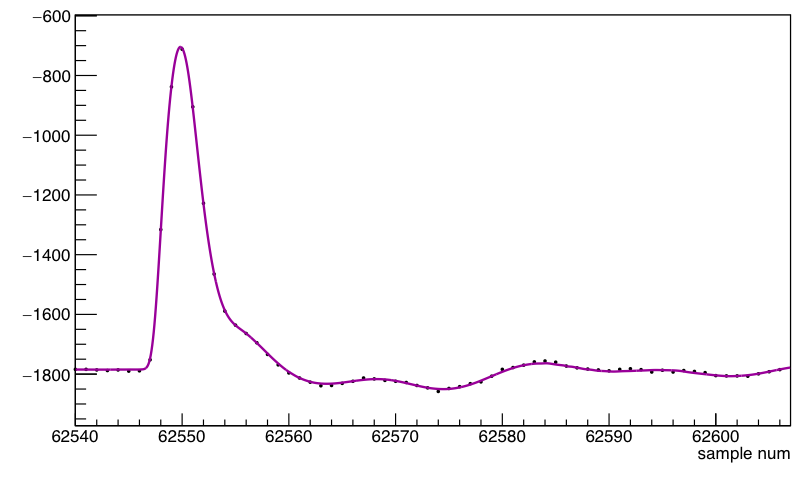
\includegraphics[width=0.6\textwidth]{hitPulse}
\caption[SiPM pulse]{Output pulse from a SiPM in black dots, overlayed with a fit template.}
\label{fig:calopulse}
\end{figure}


\subsection{Laser calibration system}
\label{sub:LaserCalibrationSystem}


In order to satisfy the gain requirements of the calorimeter detectors, a laser calibration system is used. This system monitors the SiPM responses over short and long time scales to $< 0.04\%$ \cite{Anastasi:2017sos}. The system consists of six different lasers and a suite of optical devices. The light from the six lasers is piped to a board mounted on the front face of each calorimeter through optical fibers. This board contains right-angle prisms which it uses to deflect the laser pulses directly into each calorimeter crystal, for all 1296 channels. The lasers can be pulsed at various intensities, both in-fill to monitor the STDP or IFG effects, and out-of-fill to monitor for long term drifts due to changing temperatures or detector degradation. The SiPM measured response is compared to local known source monitors in order to calibrate the SiPM energy response. Corrections to the gain of the calorimeters can thus be determined and applied to the hit energies. Simultaneously the laser system allows for measuring the timing resolution of the SiPMs, and in general performing diagnostic tests with the calorimeter. Lastly, the laser system is used to time align the different calorimeter channels by outputing a sync pulse to each channel at the beginning of every muon fill.


% older publications on tests of the laser system which I'm not sure I need to cite
% \cite{Anastasi:2015ssy} 
% \cite{Anastasi:2016luh}




\section{Straw trackers}
\label{sec:StrawTrackers}

As described in \secref{sec:muonbeamdynamics}, the muon beam moves dynamically within the storage ring. As explained in \secref{sec:MagneticField}, the muon beam distribution ties into the measurement of the magnetic field. The primary detector system used to measure this behavior and determine the muon beam distribution is the ``straw tracker'' system. The straw trackers characterize the beam in a non-destructive fashion by measuring decay positron trajectories and extrapolating back into the storage ring. They serve to provide the direct measurement of the pitch correction as described in \secref{sub:pitch_correction}, determine the momentum distribution of the beam, and characterize parameters of the CBO which tie into the calorimeter \wa analysis. Decay positron trajectories can also be extrapolated forwards into the calorimeter, in order to cross-check calorimeter measurements to help resolve pileup (be sure to talk about pileup in the calorimeter section - since this isn't actually done yet do I even want to say this?). Finally, the trackers also serve as a measuring device to search for a possible muon electric dipole moment. The existence of such a thing would tilt the precession plane of the muons and subsequent decay positron trajectories which the trackers are sensitive to. Details of the beginnings of such a search are given in \refref{SCThesis}. The details of the track reconstruction and analysis will be given in \chapref{chapter:TrackReconstruction}. Here will be given a description of the detectors themselves and how they work.


In general, straw tracking detectors work by measuring hits in gas filled straws \cite{Blum}. Each straw is made up of a cylindrical piece of thin conducting material, typically Mylar, and contains a wire at the center of the straw held at high voltage, $\mathcal{O}(\SI{1000}{V})$. The minimal amount of material in straw trackers serves to reduce multiple scattering of incident particles, and was the reason a straw tracker system was chosen over other tracker types. Fast moving particles ionize the gas as they pass through it, and the resulting ions are drawn to the wire and straw surface (positive and negative charges respectively). As the ions move to the wire, they enter a high electric field region which causes them to speed up and create more ions. This produces an avalanche gain effect to amplify the original signal. Once the ions reach the wire and straw surface, a signal is read out telling what the drift time of the ions was, which can be related to the radius or distance of closest approach (DCA) the particle passed relative to the wire. The straws therefore measure in a plane perpendicular to their physical orientation. By combining several such signals in time and space, we are able to reconstruct tracks of incident particles. See \figref{fig:driftcircles}.

\begin{figure}[]
\centering
        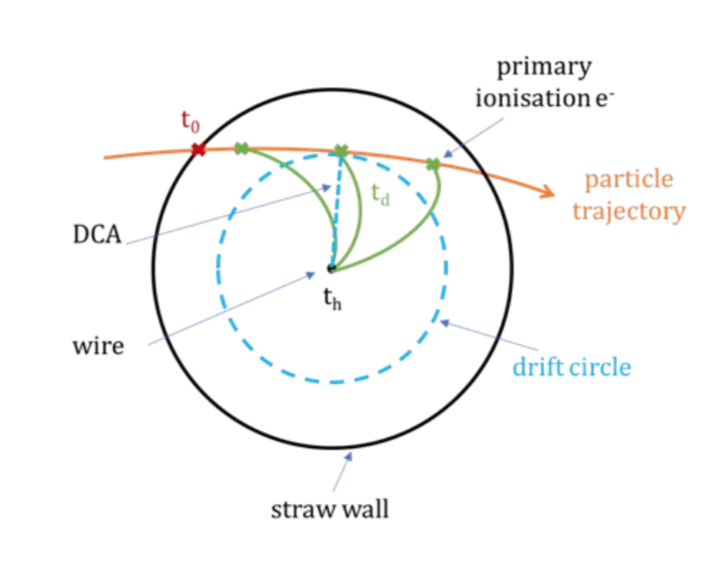
\includegraphics[width=0.6\textwidth]{StrawDriftTime}
    \hspace{1cm}
        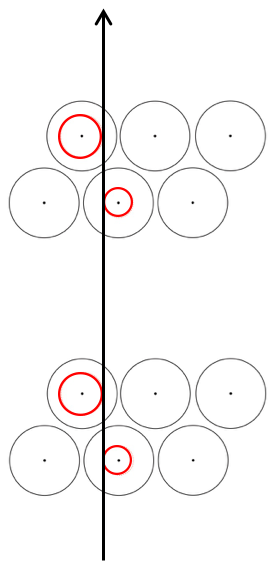
\includegraphics[width=0.25\textwidth]{TrackDriftCircles}
\caption[Straw tracker drift circles]{Diagrams showing the determination of a drift time $t_{d}$ and hit time $t_{h}$ from an incident ionizing particle (left) and the combination of several such hits to produce a track (right). Picture on left by Saskia Charity.}
\label{fig:driftcircles}
\end{figure}




Our straws are $\SI{5}{mm}$ in diameter and contain a 50:50 mixture of argon-ethane gas \cite{WTThesis}. The argon component serves as the gas to be ionized. The fast moving ions near the wire in addition to producing more ions, will incite excited states of the gas, which emit photons when de-excited. These photons can restart the whole ionization and avalanche process over again as they can escape the avalanche region, leading to a break-down of the system. The ethane therefore serves to absorb the photons with its large number of molecular degrees of freedom and photo-absorption characteristics \cite{WTThesis}. The wire has a radius of \mum{25} and is made up of gold-plated tungsten. The mylar walls have a width of \mum{15} and are wound in a double spiral shape in order to improve the electrostatic shielding of the wire and reduce the gas leak rate of the straws \cite{WTThesis}. The position resolution of hits within the straws is approximately \mum{150} \cite{something}.


\begin{figure}[]
    \centering
    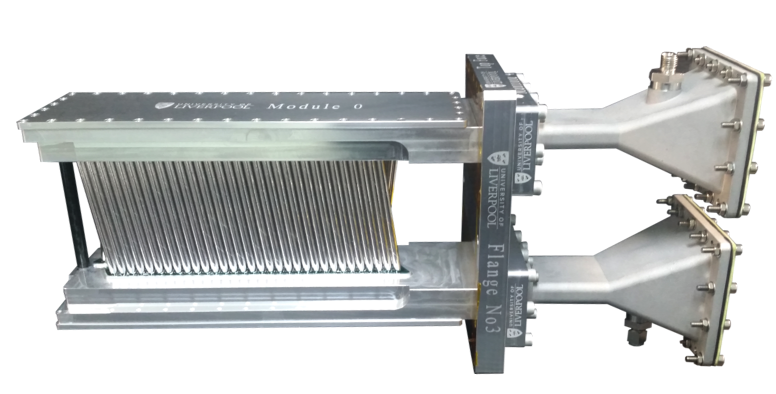
\includegraphics[width=0.9\textwidth]{Tracker}
    \caption[Tracker module]{A straw tracker module. The first layer of silver Mylar straws with a stereo angle of 7.5\textdegree{} can be seen, with the other three straw layers hiding behind it. In black on the left is the carbon fiber post which holds the end of the module in a fixed position. Electronics live in the top and bottom manifolds above and below the straws, and cables connect from those electronics through the small aperture and to external electronics which plug in on the right.}
    \label{fig:tracker}
\end{figure}



A single tracker module is shown in \figref{fig:tracker}. Each tracker module consists of four layers of thirty two straws each with stereo angles of $\pm$7.5\textdegree{}, for a total of 128 straws per module. The first two straw layers are designated as ``U'' layers, and are oriented with the tops of the straws at a greater radial position than the bottoms of the straws. The second two layers are designated as ``V'' layers, and are oriented with the bottoms of the straws at a greater radial position. See \figref{fig:trackermodulecoordsys}. The two types of layers are non-parallel to each other in order to spatially resolve incident tracks. The small stereo angle both improves the straw measurement area as electronics can be kept out of the positron decay path region, and improves the radial momentum resolution of the fitted tracks which is perhaps the most important straw tracker measurement. (Support this somehow? With a figure or text? ``The momentum resolution of both radial and vertical is about the same I believe in the extrapolation back to the storage ring.'') The active straw measurement area is approximately $\SI{10}{cm}$ high by $\SI{20}{cm}$ wide. A carbon fiber post sits at the outside end of the module to provide structural rigidity to the module, and keep the straw wires under tension. 



\begin{figure}[]
\centering
        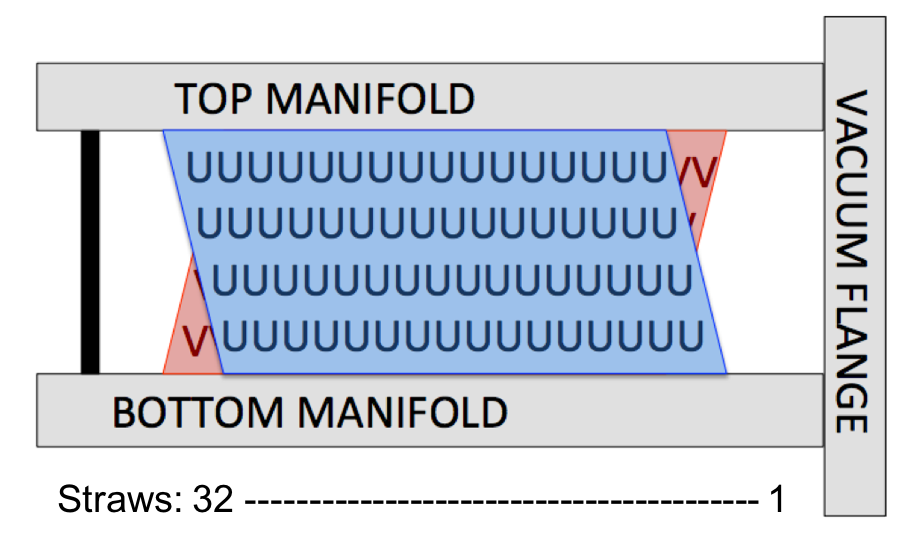
\includegraphics[width=0.6\textwidth]{straworientation_with_strawlabel}
    \hspace{1cm}
        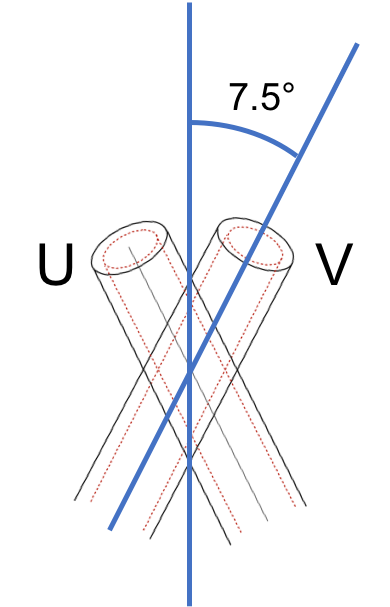
\includegraphics[width=0.25\textwidth]{StrawAngle}
\caption[Tracker module coordinate system]{Orientation of U and V straws in the tracker module.}
\label{fig:trackermodulecoordsys}
\end{figure}



There are two tracker stations, each consisting of eight tracker modules. The two stations live at positions in front of calorimeters 13 and 19, or at approximately 180\textdegree{} and 270\textdegree{} clockwise from the inflector. There is also a third station just after the inflector, which currently sits empty of any tracker modules. The straw tracker modules sit inside the vacuum chamber in specially modified vacuum chamber sections in a staircase-like pattern that follows the curvature of the ring. See \figref{fig:TrackerCaloWithLines}. The number of modules and their orientation in each station was chosen to provide a long measurement arm for precise momentum measurement of the incident tracks. The modules sit inside the vacuum in order to eliminate multiple scattering in air and produce better reconstructed tracks. Due to their proximity to the storage region, the tracker modules also live in a region of high field non-uniformity. Though the acceptances between the trackers and calorimeters are not identical, their close proximity facilitates comparison between the two measurement devices. Finally, even though the tracker stations live at only two places in the ring, they measure the average beam distribution due to the CBO motion of the beam and the long extrapolation distance of the measured trajectories.


\begin{figure}[]
    \centering
    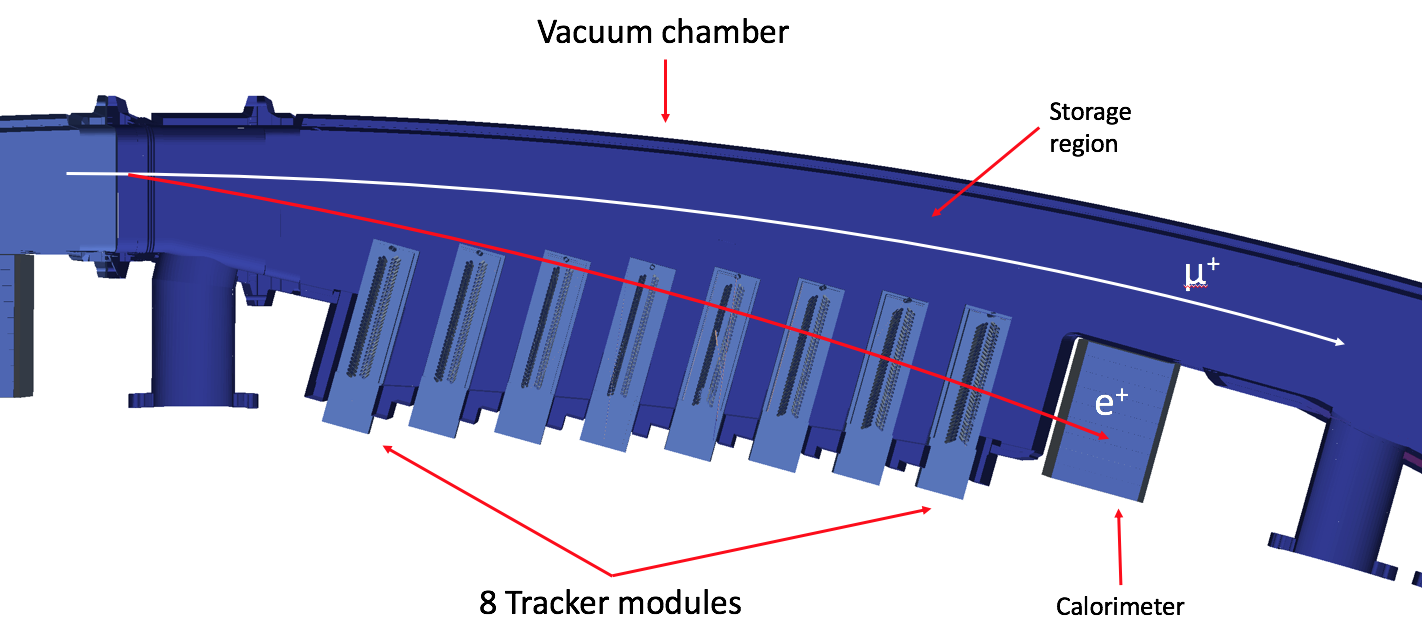
\includegraphics[width=0.9\textwidth]{TrackerCaloWithLines}
    \caption[TrackerCaloWithLines]{Birds eye view of a model of a vacuum chamber containing a tracker station, and the associated calorimeter. Each tracking station consists of 8 tracker modules.}
    \label{fig:TrackerCaloWithLines}
\end{figure}



% \begin{figure}[]
%     \centering
%     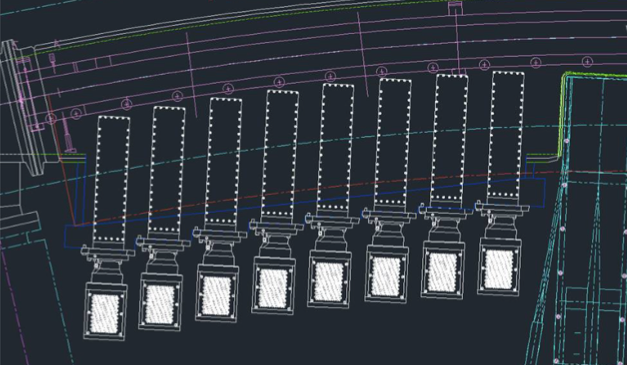
\includegraphics[width=0.9\textwidth]{trackerStation}
%     \caption[Tracker module arrangement]{Tracker modules are arranged in the shown staircase pattern. In green and dark blue is the edge of the vacuum chamber (where the dark blue identifies the modification that was made to the old vacuum chambers), and it can be seen that vacuum chamber walls lie at the ends of the outside tracking modules. The position of a calorimeter can be seen in cyan at the right. The dark red spots are the locations of the outside magnet pole tips. From the shown geometry one can see that many positrons will hit either the tracker or the calorimeter but not both due to the acceptance differences.}
%     \label{fig:staircase}
% \end{figure}


\subsection{Tracker readout electronics}


The readout electronics for the system are split into two groups, the front-end and back-end. The front-end electronics were built and tested at the Boston University Electronic Design Facility. They start with Amplifier Shaper Discriminator with charge (Q) (ASDQ) chips on boards that plug down directly onto the straws and provide the main signal. Each ASDQ plugs onto sixteen straws. These ASDQ boards are application specific integrated circuits (ASICs) which read out the signal from one end of the straws and shape and discriminate that signal, as well as providing some baseline restoration and tail cancellation. The ASDQs and their associated components live in thin aluminum manifolds above and below the straws. The physical footprint of these boards and components was minimized in order to increase the straw measurement area. The signals from the ASDQs are passed through Flexi Cables to Time to Digital Converter (TDC) boards which time stamp the signals with $\SI{625}{ps}$ precision \cite{WTThesis}. The Flexi Cables are flexible and thin such that the cables can be passed through the thin aperture shown on the right of \figref{fig:tracker}. High voltage is provided to the sense wires with high voltage boards, which pass the voltage through the ASDQs. A feedthrough board provides the interface between the TDCs and Flexi Cables, as well as the high voltage signal. They serve a dual purpose of providing the gas seal. Finally, there are logic boards that serve as the interface between the TDCs and the back-end electronics. They manage the clock and controls for the TDCs and store data onto FPGAs, which is piped out through a high throughput optical fiber connection. The logic boards, high voltage boards, and TDCs are all housed within an aluminum box which provides RF shielding. In each module there are eight ASDQs, four TDCs, two feedthrough boards, two high voltage boards, and two logic boards. An overview diagram of the front-end readout chain is shown in \figref{fig:TrackerReadoutChain}. The back-end electronics consist of FC7s, one per tracker station, and a single AMC13 for all tracker stations. These modules provide clock and DAQ services to the whole tracker system, and ultimately pipe out the data to where it can be saved on disk.


\begin{figure}[]
    \centering
    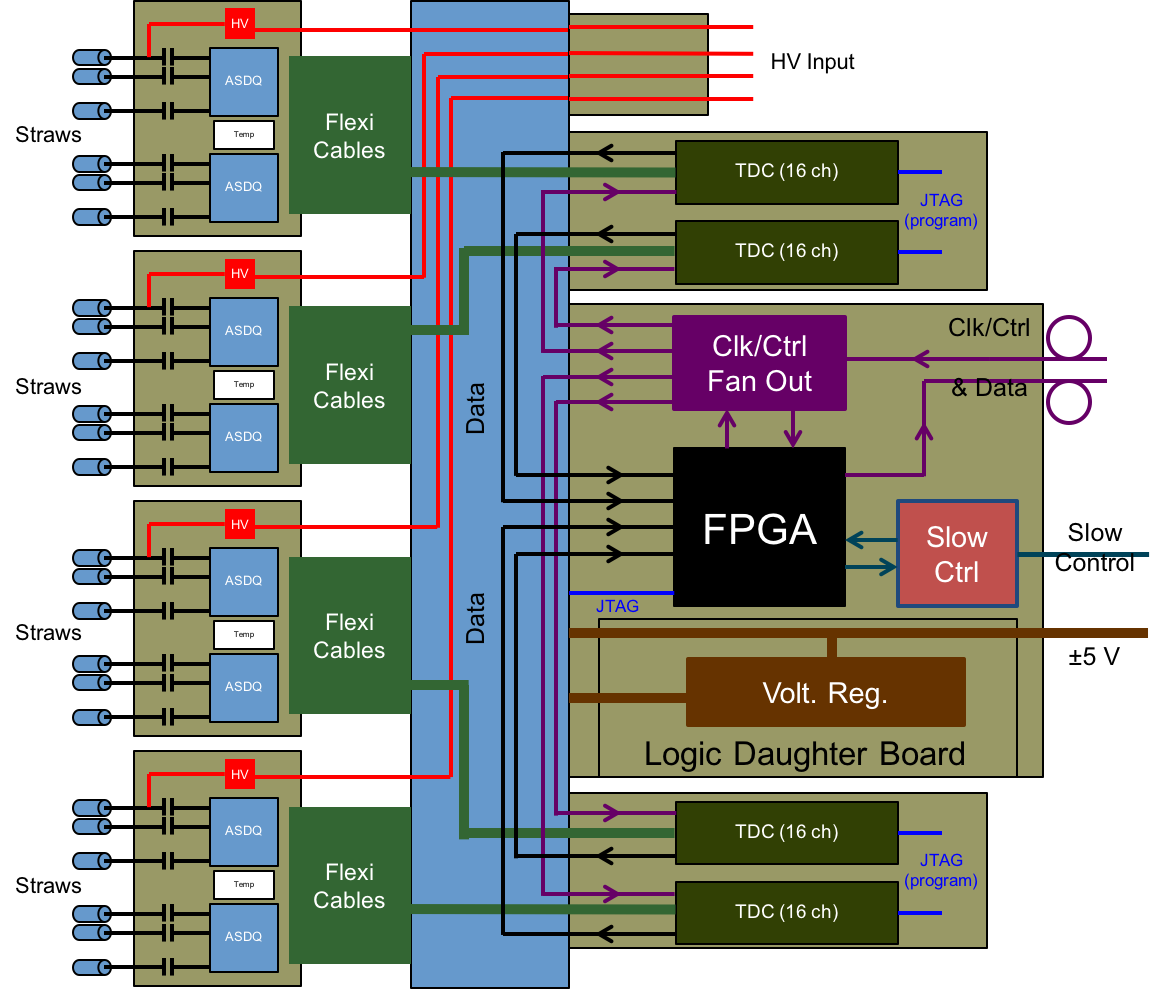
\includegraphics[width=0.9\textwidth]{TrackerReadoutChain}
    \caption[Tracker electronics readout chain]{Front-end tracker electronics readout chain. Created by James Mott.}   
    \label{fig:TrackerReadoutChain}
\end{figure}



